\begin{frame}[fragile]{Proposed Method} 
\begin{block}{Knowledge Graph (K-Graph)}
    \begin{itemize}
      \item Store object's class
      \item Store action feedback
      \item Suggest actions
    \end{itemize}
  \end{block}
\end{frame}

% \begin{frame}[fragile]{Proposed Method} 
% Formally, a \textbf{\acl{k-graph}}, $\gls{k-graph} = \left\langle \gls{nodesK}, \gls{edgesK} \right\rangle $
% \\comprising $\gls{nodesK} = \{\gls{node}^{\mathit{center}}, \gls{node}^{\mathit{side}}\}$, \quad $\gls{edgesK} \in \{\gls{edge}_{(i,j)}| i \in \gls{nodesK}^\mathit{center}_\mathit{ids}, j \in \gls{nodesK}^\mathit{side}_\mathit{ids} \}$.\bs
% \end{frame}


\begin{frame}[fragile]{Proposed Method} 
  Success Factor \bs

  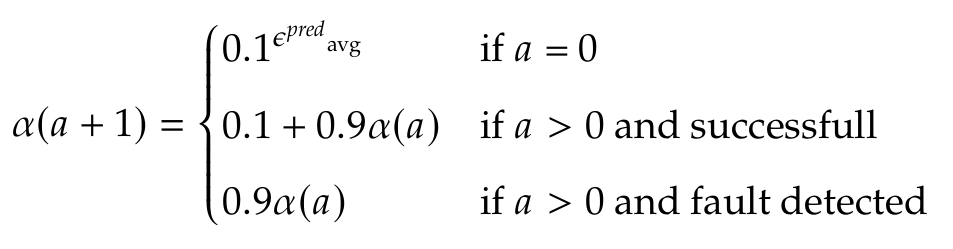
\includegraphics[width=0.6\textwidth]{figures/proposed_method/successfactor}

% Formally the \textbf{success factor} = \gls{successfactor}:
% \begin{equation}
% \gls{successfactor}(a+1) =
%   \begin{cases} 0.1^{\gls{pe}_\textrm{avg}}& \textrm{if $a$ = 0}\\[5px]
%     0.1 + 0.9\gls{successfactor}(a) & \textrm{if $a > 0$ and the reviewed edge was successfully completed}\\[5px]
%   0.9\gls{successfactor}(a) & \textrm{if $a > 0$ and the reviewed edge failed during execution time}
% \end{cases}
% \label{eq:success_factor}
% \end{equation}
\end{frame}

% \begin{frame}[fragile]{Proposed Method} 
% \end{frame}

% \begin{frame}[fragile]{Proposed Method} 
% \end{frame}
